\customchapter{Description of the Design Elements}
\section{Register file design}

In a RISC-V processor architecture, the register file typically consists of a set of general-purpose registers (GPRs) used for temporary storage of data during program execution. 

\subsection{RISC-V compatibility } 

For the register file to be RISC-V compatible the typical IO ports of the register file would be A1, A2, A3, WD3, RD1, RD2, RST, REGWR and CLK as shown in the below figure 6.1. Here A1, A2 and A3 are 5-bit register addresses. A1 and A2 are the addresses of the read registers and A3 is the address of the write register. RD1, RD2 and WD3 are 32-bit registers. REGWR is 1-bit enable pins which enables write operation. CLK is the clock signal as the register file is a synchronous block. RST is a reset 1-bit reset signal.

\subsection{Write Operation} 

The data that needs to be written into the register file is written into the 32-bit WD3 register and the location of the write operation is determined by the 5-bit A3 register. Upon every rising edge of the clock cycle when the REGWR is high the data present in the WD3 register is written into the corresponding register determined by the address present in A3 of the register file.

\subsection{Read Operation} 

RD1 and RD2 registers hold the data that is read from the registers of the register file based on the addresses present in A1 and A2 respectively. Read operation is an asynchronous operation.

\subsection{Scan Flip Flop} 

To make the register file scan testable every register of the register file is designed with scan flip-flops. The architecture of the scan chain-enabled register file will be further described in section 7.1.
The RISC-V instruction set architecture uses a CPU register file with 32x 32-bit registers named R0 through R31. Instructions encode register addresses as 5-bit fields within the instruction binary number using names such as Rs1, Rs2 and Rd. These address bitfields are connected to three address inputs of the register file. Address A1 selects the register to output as RD1 and become input A of the ALU. Address A2 selects the register to output as RD2 and potentially becomes input B of the ALU. Address A3 selects which register should store the data calculated by the circuit if the controller commands a store using the REGWR control signal. Figure 6.1 shows the register file which can be interfaced with the Arithmetic Logic Unit.




\begin{figure}[h] % Use the 'h' option to try to place the image "here"
  \centering
  \setlength{\abovecaptionskip}{-10pt} % Reduce space above the caption
  \setlength{\belowcaptionskip}{0pt} % Adjust space below the caption
  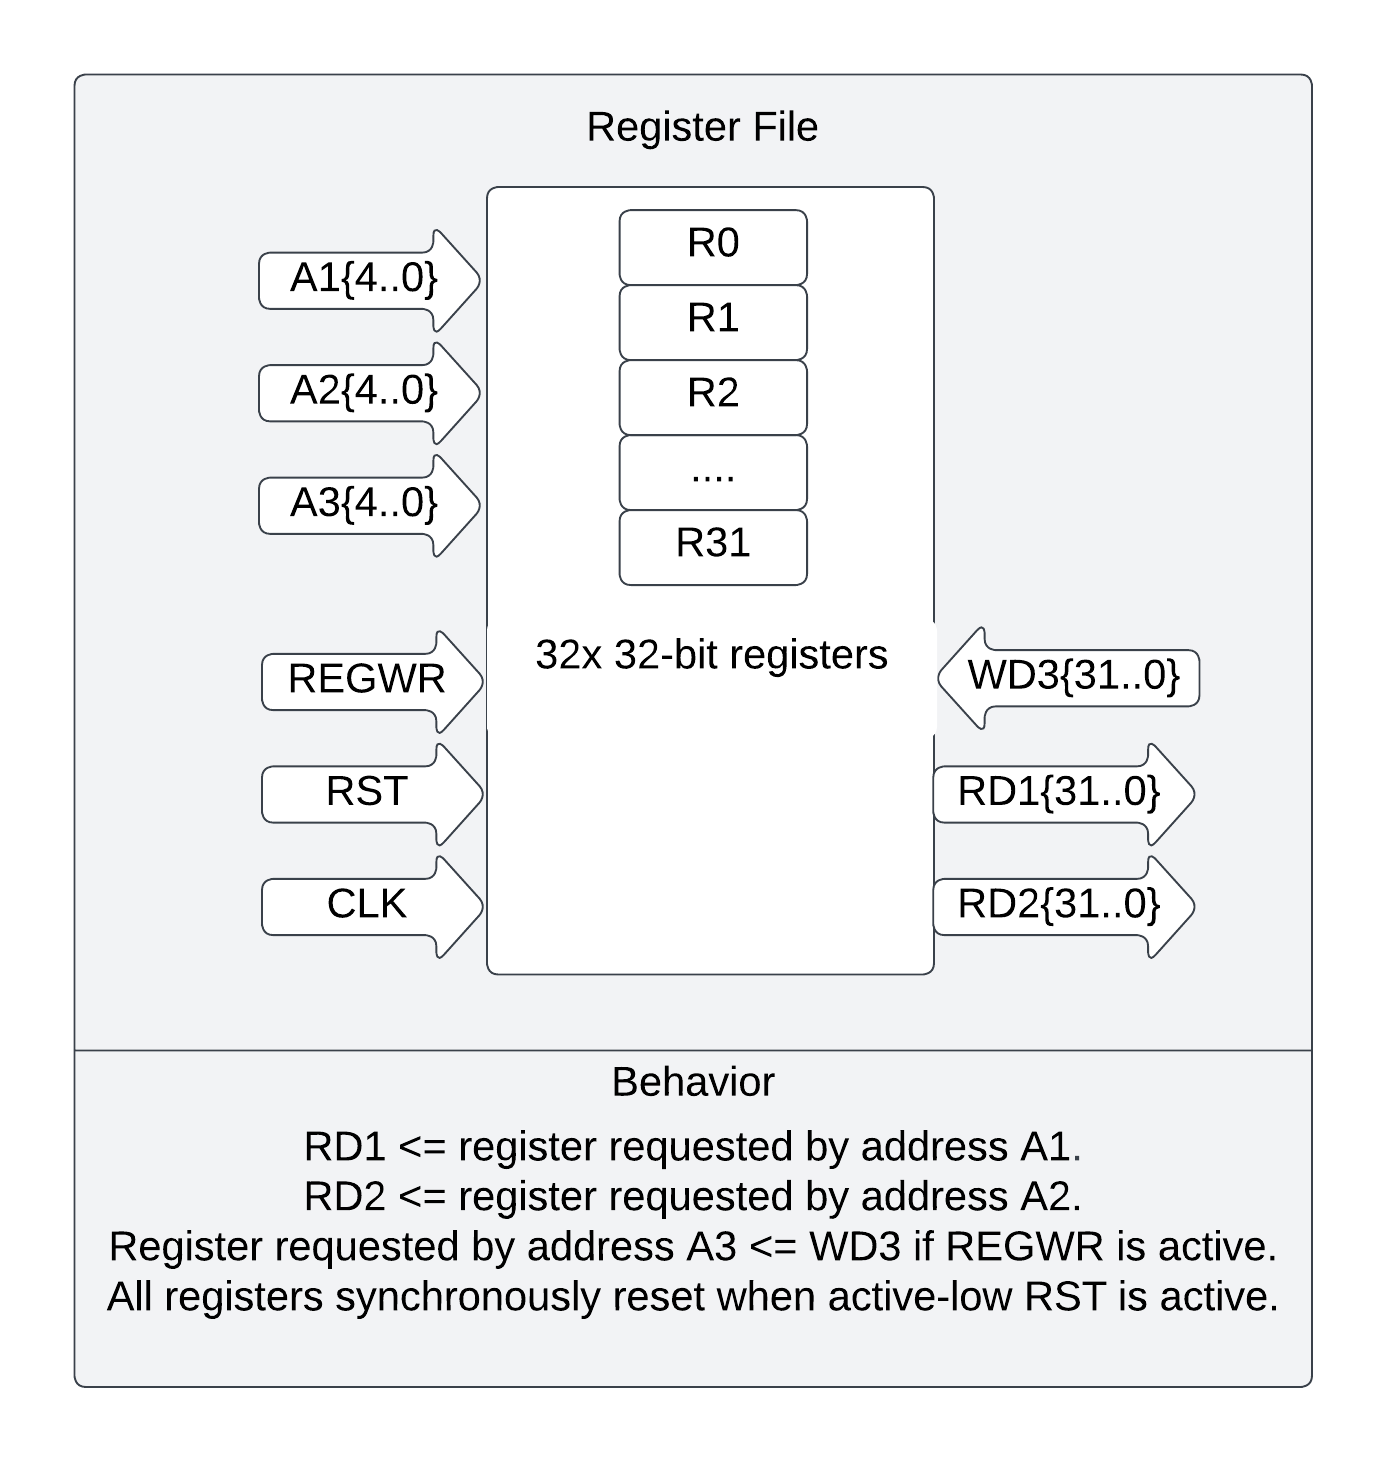
\includegraphics[width=0.6\textwidth]{Image/Register.png} % Replace 'your-image.png' with the actual file name
  \caption{Register File}
  \label{Figure 1 : Register File}
\end{figure}


\pagebreak
\newpage
\section{TAP Controller}
The Test Access Port (TAP) controller, as defined by the IEEE Std. 1149.1 standard, plays a crucial role in enhancing the efficiency of testing procedures for integrated circuits. The IEEE Std. 1149.1, commonly known as Boundary-Scan Testing, establishes a standardized approach for testing and debugging digital circuits. This standard introduces the TAP controller, a fundamental component in the implementation of the Boundary-Scan architecture.
\vspace{3mm}

\textbf{TAP Controller Overview:}
The TAP controller serves as the primary interface between the external testing equipment and the internal components of an integrated circuit. It facilitates communication and control during the testing process, enabling the execution of various test patterns and configurations.
\vspace{2mm}

\textbf{Key features of the TAP controller include:}
\vspace{2mm}

\hspace{4mm} Test Access Port (TAP): The TAP comprises a series of standardized instructions and registers that allow external devices, such as Automatic Test Equipment (ATE), to communicate with and control the internal components of a digital circuit.
\vspace{2mm}

\hspace{4mm}Shift Register Mechanism: The TAP controller utilizes a shift register mechanism to capture, shift, and update data within the integrated circuit. This mechanism enables the testing of individual components and the observation of their responses.
\vspace{2mm}

\hspace{4mm}Instruction Register: The TAP controller incorporates an instruction register that holds a set of instructions for testing specific components or performing specific operations within the circuit. These instructions are standardized by the IEEE Std. 1149.1.
\vspace{2mm}
\newpage
\subsection{IEEE Std. 1149.1 Scan Testing:}

\textbf{Key components of IEEE Std. 1149.1 Scan Testing include:}
\vspace{2mm}

\textbf{Scan Register :} This register surrounds each digital component and provides a means to observe and control the signals at the component's boundary. This allows for the serial testing of interconnected components.
\vspace{2mm}

\textbf{Scan Cells:} These cells, integrated into the design of digital components, enable the capture and observation of data at the component's input and output pins. These cells facilitate the testing of connections and components on the PCB.
\vspace{2mm}

\textbf{Standardized Instructions:} IEEE Std. 1149.1 defines a set of standardized instructions that the TAP controller uses to perform various operations, such as entering and exiting test modes, shifting data in and out of the Scan register, and executing test patterns.
\vspace{2mm}

\textbf{TAP Controller Architecture:}

The boundary-scan circuitry can be divided into four main hardware components: 
\vspace{1mm}

\begin{itemize}
    \item A test access port (TAP), which consists of four mandatory terminals test data input (TDI), test data output (TDO), test mode select (TMS), and test clock (TCK) and one optional terminal, test reset (TRST).
    \item A TAP controller (TAPC).
    \item An instruction register (IR) and its associated decoder.
    \item Several test data registers, including the mandatory boundary-scan register and bypass register, and some optional miscellaneous registers, such as the device-ID register, and some design-specific test data registers.
\end{itemize}

\begin{figure}[h] % Use the 'h' option to try to place the image "here"
  \centering
  \setlength{\abovecaptionskip}{0pt} % Reduce space above the caption
  \setlength{\belowcaptionskip}{0pt} % Adjust space below the caption
  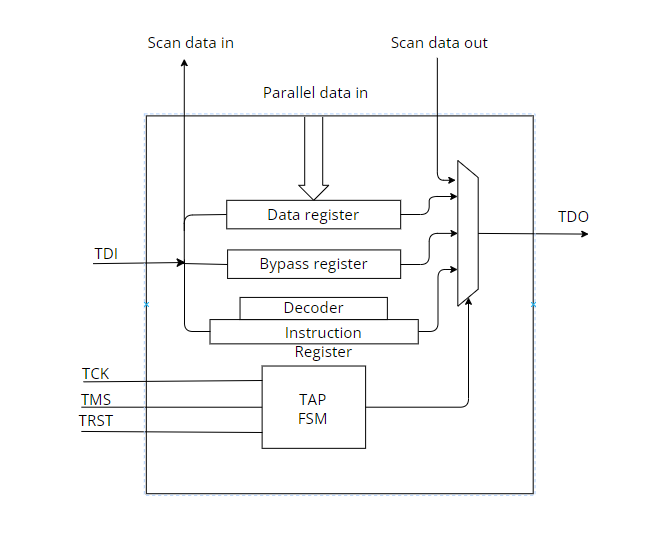
\includegraphics[width=0.7\textwidth]{Image/TAP1.png} % Replace 'your-image.png' with the actual file name
  \caption{TAP Controller Architecture}
  \label{Figure 6.3 : ARM Cortex-A9}
\end{figure}

TAP Controller architecture in IEEE Std. 1149.1 requires serial loading of instructions into the instruction register via the TDI pin. The associated decoder generates test signals for configuring hardware. Test data registers store data or system-related info. IEEE Std. 1149.1 defines instructions like BYPASS, SAMPLE, PRELOAD. The typical test procedure involves shifting a test instruction into the IR, decoding it to configure logic, applying a test pattern, capturing the response in a data register, observing via TDO, and repeating for all test patterns.
As per the implementation in project the TapController\_e entity defines the input and output ports of the TAP controller. These include inputs such as TDK (Test Clock), TMS (Test Mode Select), TDI (Test Data In), TRST (Test Reset), and parallel\_data\_in (Parallel Data In). Outputs include TDO (Test Data Out), scan\_in\_data (Scan In Data), and scan\_out\_data (Scan Out Data).
The first process handles the state transitions of the TAP controller based on the rising edge of the test clock (TCK) and the test mode select (TMS) signals. The second process is responsible for the actual implementation of the TAP controller's functionality based on its current state.
\vspace{5mm}

\subsection{TAP FSM:}
The TAP controller operates based on a Finite State Machine (FSM) that defines different states for the testing process. These states include Test\_Logic\_Reset, Run\_Test\_Idle, Select\_DR\_Scan, Capture\_DR, Shift\_DR, Exit1\_DR, Pause\_DR, Exit2\_DR, Update\_DR, Select\_IR\_Scan, Capture\_IR, Shift\_IR, Exit1\_IR, Pause\_IR, Exit2\_IR, and Update\_IR. Transitions between states are based on the values of the TMS signal.
\vspace{3mm}

\begin{figure}[h]
    \centering
    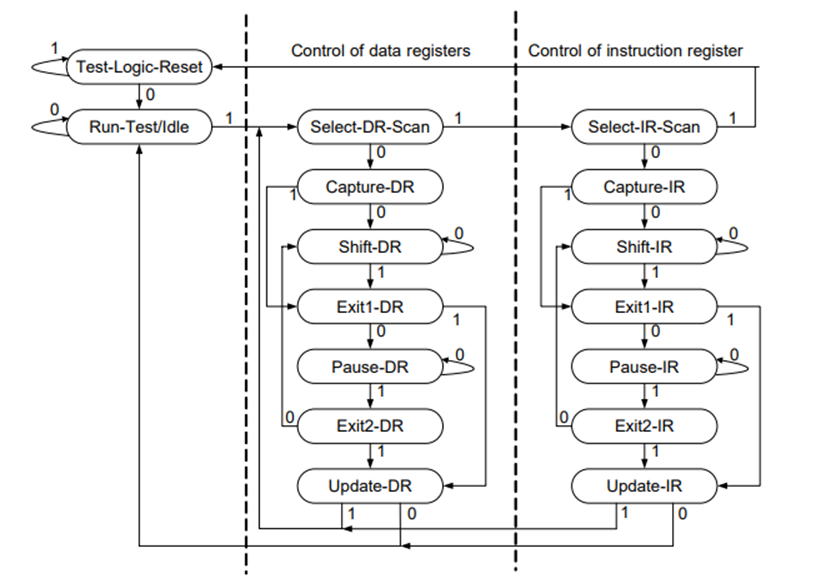
\includegraphics[width=0.9\linewidth]{Image/FSM.png}
    \caption{Finite State Machine}
    \label{fig:enter-label}
\end{figure}

The FSM guides the TAP controller through a sequence of steps, ensuring the proper execution of test instructions and the capture of test responses. It plays a crucial role in coordinating the testing process, from loading instructions into registers to shifting data and updating internal states. Together, the TAP controller and FSM form a standardized approach to boundary-scan testing, enhancing the efficiency and reliability of digital circuit testing procedures.
\vspace{3mm}

\newpage
\subsection{\textbf{Data Register:}}
\begin{figure}[h]
    \centering
    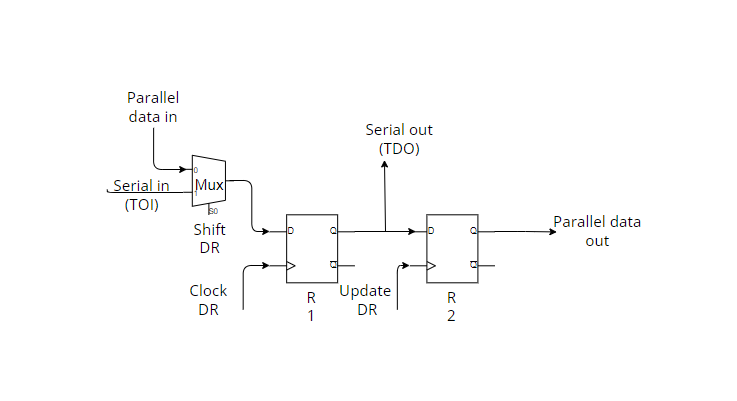
\includegraphics[width=1\linewidth]{Image/dataregister.png}
    \caption{Data Register}
    \label{fig:enter-label}
\end{figure}
In normal mode (Mode = 0), data flows directly from IN to OUT, and the cell is transparent to functional logic. In Test mode (Mode = 1), test data from the dr2 flip-flop passes through a multiplexer to the OUT signal. TAP controller signals (ClockDR, ShiftDR, UpdateDR) control three main test operations: Capture, Shift, and Update. During Capture, data at IN is captured into D-FF dr1. In Shift, test data is shifted in from SI, and the test response is scanned out through SO. Update propagates dr1 data to dr2. If Mode is 1, dr2 output connects to OUT. Capture and Shift operations can also occur in normal mode. Test data can be latched in dr2 (and OUT if Mode = 1) while other data is shifted in/out.
\vspace{3mm}

\subsection{\textbf{Instruction Registration:}}

The Instruction Register (IR) stores the instruction to be executed in a two-stage(ir1 and ir2) design same as data register, preventing indeterminate states during instruction shifting. Four mandatory boundary-scan test instructions (SAMPLE, PRELOAD, BYPASS, EXTEST) are defined in IEEE Std. 1149.1.
\vspace{3mm}

\subsection{\textbf{Parallel and Serial Data Handling:}}
The code includes the handling of parallel data (parallel\_data\_in, parallel\_data\_out) and serial data (TDI, TDO) based on the current state of the TAP controller.
Shift and capture operations are performed on the dr1 and ir1 signals.
\vspace{2mm}

[Note : As per the implementation, Parallel input is taken from registers and Parallel output is not being used, it kept as open to use in future.]
\vspace{3mm}

\subsection{\textbf{Update Operations:}}
Update operations are handled for both the instruction register (ir2) and the data register (dr2).
The TAP controller shifts the updated data into the respective registers.
\vspace{3mm}
\newpage
\subsection{\textbf{TAP Controller Tests:}}
\textbf{Scan Chain:}
The code includes handling for the Scan Chain operation, allowing data to be shifted in and out through the scan\_in\_data and scan\_out\_data signals.
\vspace{1mm}

\textbf{Bypass Handling:}
Bypass functionality is also implemented, allowing the TAP controller to bypass the internal circuitry and directly pass the data through.
\vspace{1mm}

\textbf{Sample:}
During the rising edge of the test clock (TCK), if the test reset is not active, the parallel data from parallel\_data\_in is loaded into dr1.
This captures the input data at the parallel input into the data register for subsequent testing operations.
\vspace{1mm}

\textbf{Preload:}
The "Preload" operation shifts and updates data, sending the MSB to TDO and preparing the register for the next bit with TDI.
Test Reset (TRST) Handling:
The code includes logic to reset the internal registers (dr1, dr2, ir1, ir2) when the test reset signal (TRST) is asserted.
\vspace{1mm}

\section{Target SoC Architecture}
\begin{figure}[h] % Use the 'h' option to try to place the image "here"
  \centering
  \setlength{\abovecaptionskip}{0pt} % Reduce space above the caption
  \setlength{\belowcaptionskip}{0pt} % Adjust space below the caption
  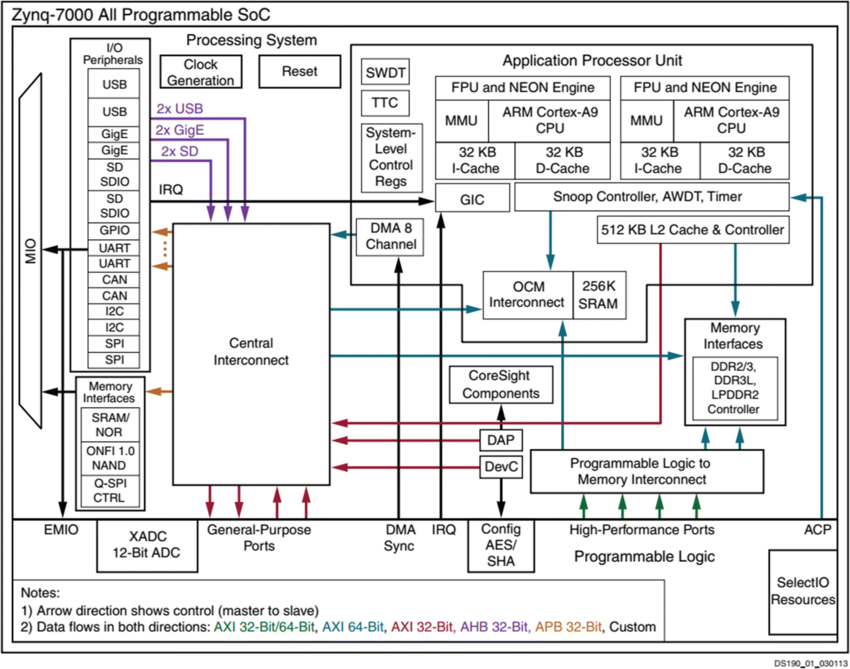
\includegraphics[width=0.8\textwidth]{Image/soc7000.png} % Replace 'your-image.png' with the actual file name
  \caption{Architecture overview}
  \label{Figure 1 : Architecture overview}
\end{figure}

Xilinx Zynq-7000 SoC allows a flexible platform to launch solutions while providing traditional SoC users with a fully programmable alternative. The Arm Cortex-A9 processor present provides an integrated processing system (PS). The XA Zynq-7000 architecture enables the implementation of custom logic in the PL and custom software in the PS. 
\vspace{2mm}
\\
The PS comprises four major blocks Application processor unit (Two dual-core ARM Cortex-A9 processors), Interconnect, I/O peripherals and Memory interfaces. The APU, memory interface unit and I/O peripherals are all connected to each other and to the PL through an ARM AMBA AXI interconnect. The interconnect is non-blocking and supports multiple simultaneous master-slave transactions.
\\

\vspace{2mm}
In the scope of our SoC, the custom synthesised IP’s (Register file, TAPC) will be deployed into the PL section of Xilinx Zynq-7000 SoC and these IP’s will be interfaced with the PS (ARM Cortex APU) via an AXI interconnect.

\section{ARM Core}
The Cortex-A9 is a multi-core microprocessor that uses a dual-issue, in-order pipeline design. It features various architectural enhancements over its predecessor, the Cortex-A8, resulting in improved performance and energy efficiency. The Cortex-A9 uses the ARMv7-A instruction set architecture, which supports both 32-bit and 64-bit instruction sets. This architecture is widely used in modern ARM-based processors. 

\begin{figure}[h] % Use the 'h' option to try to place the image "here"
  \centering
  \setlength{\abovecaptionskip}{0pt} % Reduce space above the caption
  \setlength{\belowcaptionskip}{0pt} % Adjust space below the caption
  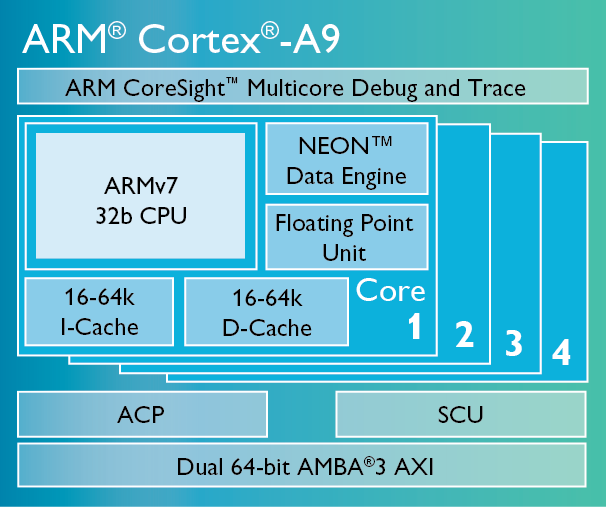
\includegraphics[width=0.5\textwidth]{Image/ARM core.png} % Replace 'your-image.png' with the actual file name
  \caption{ARM Cortex-A9}
  \label{Figure 1 : ARM Cortex-A9}
\end{figure}


The Cortex-A9 can be configured as a single-core or multi-core processor. It is often used in multi-core configurations, which can provide increased processing power for more demanding applications. The Cortex-A9 is capable of delivering strong performance for a wide range of applications, including smartphones, tablets, networking equipment, automotive infotainment systems, and more. Its performance can be further enhanced in multi-core
configurations. The Cortex-A9 is available in a form that can be implemented in Field-Programmable Gate Arrays (FPGAs). This allows for hardware acceleration and customization in embedded systems and specialized applications.